\chapter{Zezat's Fleet}

\vspace{\baselineskip}

\begin{paracol}{2}

\begin{enumerate}
    \item Use the switch to enter the castle
    \item Go to Cara in the bedroom
    \item Go to Hiryuu on the rooftop
    \item Head northeast to the nearby island
\end{enumerate}

\switchcolumn
\begin{misc}{Path to Zezat's Fleet}
    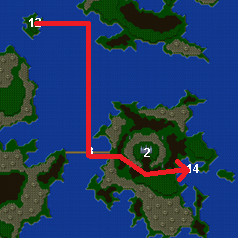
\includegraphics[scale=0.7]{../Graphics/Maps/11. To Zezat's Fleet.png}
\end{misc}

\switchcolumn*
\begin{enumerate}[resume]
    \item Head below deck and enter the room on the right
\end{enumerate}

\begin{boss}{Gabbledeak}
	\varwb
    \begin{notes}
        \item \bossHl{Kunai is the right weapon}
    \end{notes}
	\begin{round}{1}
		\faris Item \then \unequip{\kunai} \then Put near the bottom \then \battleGroup{Defend}
        \galuf Defend
        \bartz \leftCommand{\gilToss}
	\end{round}
	\varwe
\end{boss}

\switchcolumn
\begin{misc}{Menu Here}
    \insertScreenshot{../Graphics/Misc/16. Gilgamesh 3 Menu.png}
\end{misc}

\switchcolumn
\begin{menu}{Before Interacting with Gilgamesh}
    \varwb
    \begin{itemMenu}
        \hiPotionMenu \ally{Anyone low on HP}
    \end{itemMenu}
    \begin{jobMenu}
        \bartz Chemist \textbf{(\pointUp)(\pointRight)} \ability{!\gilToss} \optimize
        \galuf Time Mage \textbf{(2\pointLeft)(\pointUp)}
    \end{jobMenu}
    \varwe
\end{menu}

\begin{boss}{Gilgamesh}
	\varwb
	\begin{round}{1}
		\faris \hiPotion \space \then \ally{Faris}
        \bartz Defend
        \lenna \leftCommand{\release}
        \item \bossMenu{Group Combine items together}
        \item \bossMenu{\textbf{Revivify} \mbox{\switch}\textbf{Maiden's Kiss}}
        \item \bossMenu{\textbf{Antidote} \mbox{\switch}\textbf{Phoenix Down}}
        \item \bossMenu{\textbf{Eyedrop}}
        \vspace{1mm}
        \item[] \insertBattleMenu{../Graphics/Battle/9. Gilgamesh 2 Menu.png}
	\end{round}
    \begin{bossPart}{If Death Misses}
        \galuf \leftCommand{\dimenAbility} \then \reset
    \end{bossPart}
	\varwe
\end{boss}

\begin{menu}{After Gilgamesh}
    \varwb
    \begin{jobMenu}
        \galuf Thief \textbf{(2\pointRight)} \ability{!\escape}
    \end{jobMenu}
    \varwe
\end{menu}

\begin{enumerate}[resume]
    \item Head below deck and enter the room on the left
\end{enumerate}

\end{paracol}